\section{NEW LAX SOD PLOTS}
All domains are $[-5, 5]$, we set the end time $T=1.5$, used $3000$ samples.
\section{The Sod Shock Tube}
\subsection{Problem description}

1D Euler, $\gamma=1.4$, two states: 
We let the left state be given as
\begin{align*}
\rho_L&\sim \U[0.3, 1.2]\\
w_L&\sim \U[0, 1]\\
p_L&\sim\U[0.9, 4.1]
\end{align*}
and the right state
\begin{align*}
\rho_R&\sim \U[0.1, 0.7]\\
w_R&=0\\
p_R&\sim \U[0.05, 0.7].
\end{align*}
The shock location is given as $X\sim \U[-0.5, 0.5]$. 

Training data on 128 QMC points. mesh resolution 2048. Total validation samples: 16256



\begin{figure}
	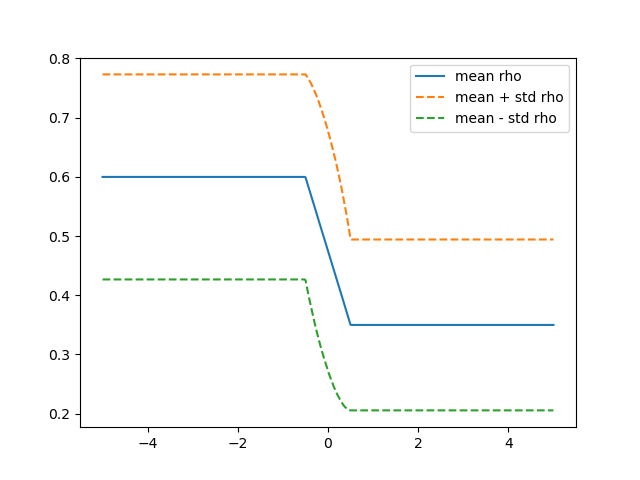
\includegraphics[width=0.8\textwidth]{img/rho_mean_std_0}
	
	\caption{$\rho$ at $t=0$.}
\end{figure}

\begin{figure}
	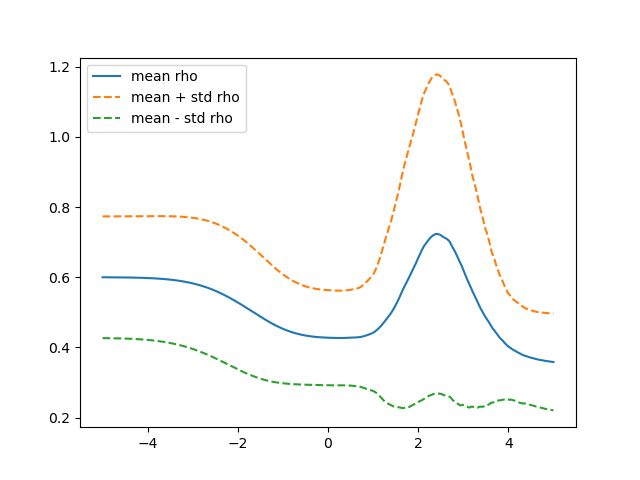
\includegraphics[width=0.8\textwidth]{img/rho_mean_std_1}
	
	\caption{$\rho$ at $t=1.5$.}
\end{figure}

%%%%%%%%%%%%%%%%%%%%%%%%%%%%%%%%%%%%%%%%%
\begin{figure}
	\includegraphics[width=0.8\textwidth]{img/mx_mean_std_0}
	
	\caption{$m_x$ at $t=0$.}
\end{figure}

\begin{figure}
	\includegraphics[width=0.8\textwidth]{img/mx_mean_std_1}
	
	\caption{$m_x$ at $t=1.5$.}
\end{figure}

%%%%%%%%%%%%%%%%%%%%%%%%%%%%%%%%%%%%%%%%%

\begin{figure}
	\includegraphics[width=0.8\textwidth]{img/E_mean_std_0}
	
	\caption{$E$ at $t=0$.}
\end{figure}

\begin{figure}
	\includegraphics[width=0.8\textwidth]{img/E_mean_std_1}
	
	\caption{$E$ at $t=1.5$.}
\end{figure}

%%%%%%%%%%%%%%%%%%%%%%%%%%%%%%%%%%%%%%%%%%%

\begin{figure}
	\includegraphics[width=0.8\textwidth]{img/p_mean_std_0}
	
	\caption{$p$ at $t=0$.}
\end{figure}

\begin{figure}
	\includegraphics[width=0.8\textwidth]{img/p_mean_std_1}
	
	\caption{$p$ at $t=1.5$.}
\end{figure}




\begin{figure}
	\subfigure[$Q_1$]{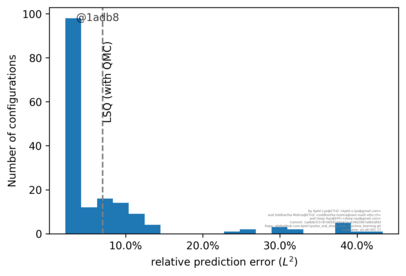
\includegraphics[width=0.5\textwidth]{img/laxsodhist_prediction_l2_relative_q1_allconfigurationsbestperforming_128_ordinary_notitle.png}}
	\subfigure[$Q_2$]{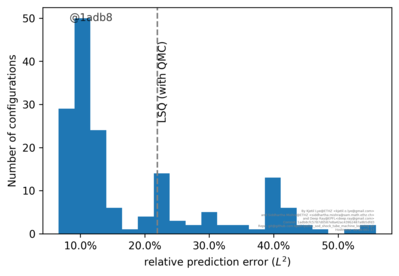
\includegraphics[width=0.5\textwidth]{img/laxsodhist_prediction_l2_relative_q2_allconfigurationsbestperforming_128_ordinary_notitle.png}}
	\subfigure[$Q_3$]{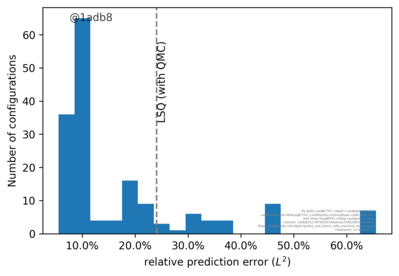
\includegraphics[width=0.5\textwidth]{img/laxsodhist_prediction_l2_relative_q3_allconfigurationsbestperforming_128_ordinary_notitle.png}}
	\caption{lax sod histogram all configurations.}

\end{figure}

\begin{figure}
	\subfigure[$Q_1$]{\includegraphics[width=0.48\textwidth]{img/laxsodcomparison_histogram_prediction_l2_relative_q1_sgd_adam_128_ordinary_bestperforming_notitle.png}} 
	\subfigure[$Q_2$]{\includegraphics[width=0.48\textwidth]{img/laxsodcomparison_histogram_prediction_l2_relative_q2_sgd_adam_128_ordinary_bestperforming_notitle.png}} 
	\subfigure[$Q_3$]{\includegraphics[width=0.48\textwidth]{img/laxsodcomparison_histogram_prediction_l2_relative_q3_sgd_adam_128_ordinary_bestperforming_notitle.png}} 
	\caption{Histograms for the relative prediction errors comparing the ADAM and SGD algorithms on the lax sod shock tube}
	
\end{figure}


%%%%%%%%%%%%%%%%%%%%%%%%%%%%%%%%


\begin{figure}
	\subfigure[Q1]{\includegraphics[width=0.48\textwidth]{img/laxsodcomparison_histogram_prediction_l2_relative_q1_goodadam_badadam_128_ordinary_bestperforming_notitle.png}}
	\subfigure[Q2]{\includegraphics[width=0.48\textwidth]{img/laxsodcomparison_histogram_prediction_l2_relative_q2_goodadam_badadam_128_ordinary_bestperforming_notitle.png}}
	\subfigure[Q3]{\includegraphics[width=0.48\textwidth]{img/laxsodcomparison_histogram_prediction_l2_relative_q3_goodadam_badadam_128_ordinary_bestperforming_notitle.png}}
	\caption{Histograms of the relative prediction errors, comparing \emph{Good} ADAM and \emph{bad} ADAM, for the LAX SOD.}

\end{figure}

\begin{figure}
	\subfigure[Q1]{\includegraphics[width=0.48\textwidth]{img/laxsodcomparison_histogram_prediction_l2_relative_q1_goodadammse_goodadammae_128_ordinary_bestperforming_notitle.png}}
	\subfigure[Q2]{\includegraphics[width=0.48\textwidth]{img/laxsodcomparison_histogram_prediction_l2_relative_q2_goodadammse_goodadammae_128_ordinary_bestperforming_notitle.png}}
	\subfigure[Q3]{\includegraphics[width=0.48\textwidth]{img/laxsodcomparison_histogram_prediction_l2_relative_q3_goodadammse_goodadammae_128_ordinary_bestperforming_notitle.png}}
	\caption{Histograms for the relative prediction errors, comparing the mean absolute error and mean square error loss functions, for theLAX SOD}

\end{figure}

%%%%%%%%%%%%%%%%%%%%%%%%%%%%%



\begin{figure}
	\subfigure[Q1]{\includegraphics[width=0.48\textwidth]{img/laxsodcomparison_histogram_prediction_l2_relative_q1_goodadaml1reg_goodadaml2reg_128_ordinary_bestperforming_notitle.png}}
	\subfigure[Q2]{\includegraphics[width=0.48\textwidth]{img/laxsodcomparison_histogram_prediction_l2_relative_q2_goodadaml1reg_goodadaml2reg_128_ordinary_bestperforming_notitle.png}}
	\subfigure[Q3]{\includegraphics[width=0.48\textwidth]{img/laxsodcomparison_histogram_prediction_l2_relative_q3_goodadaml1reg_goodadaml2reg_128_ordinary_bestperforming_notitle.png}}
	\caption{Histograms for the relative prediction error, comparing $L^1$ and $L^2$ regularizations of the loss function, for the LAX SOD}
	\label{fig:afoilreg}
\end{figure}

\begin{figure}
	\subfigure[Q1]{\includegraphics[width=0.32\textwidth]{img/laxsodcomparison_histogram_prediction_l2_relative_q1_goodadamwithval_goodadamwithwasstrain_128_ordinary_bestperforming_notitle.png}} 
	\subfigure[Q1]{\includegraphics[width=0.32\textwidth]{img/laxsodcomparison_histogram_prediction_l2_relative_q1_goodadamwithtrain_goodadamwithwasstrain_128_ordinary_bestperforming_notitle.png}}
	\subfigure[Q1]{\includegraphics[width=0.32\textwidth]{img/laxsodcomparison_histogram_prediction_l2_relative_q1_goodadamwithmeantrain_goodadamwithwasstrain_128_ordinary_bestperforming_notitle.png}}
	\subfigure[Q2]{\includegraphics[width=0.32\textwidth]{img/laxsodcomparison_histogram_prediction_l2_relative_q2_goodadamwithval_goodadamwithwasstrain_128_ordinary_bestperforming_notitle.png}} 
	\subfigure[Q2]{\includegraphics[width=0.32\textwidth]{img/laxsodcomparison_histogram_prediction_l2_relative_q2_goodadamwithtrain_goodadamwithwasstrain_128_ordinary_bestperforming_notitle.png}}
	\subfigure[Q2]{\includegraphics[width=0.32\textwidth]{img/laxsodcomparison_histogram_prediction_l2_relative_q2_goodadamwithmeantrain_goodadamwithwasstrain_128_ordinary_bestperforming_notitle.png}}
	\subfigure[Q3]{\includegraphics[width=0.32\textwidth]{img/laxsodcomparison_histogram_prediction_l2_relative_q3_goodadamwithval_goodadamwithwasstrain_128_ordinary_bestperforming_notitle.png}} 
	\subfigure[Q3]{\includegraphics[width=0.32\textwidth]{img/laxsodcomparison_histogram_prediction_l2_relative_q3_goodadamwithtrain_goodadamwithwasstrain_128_ordinary_bestperforming_notitle.png}}
	\subfigure[Q3]{\includegraphics[width=0.32\textwidth]{img/laxsodcomparison_histogram_prediction_l2_relative_q3_goodadamwithmeantrain_goodadamwithwasstrain_128_ordinary_bestperforming_notitle.png}}
	\caption{LAX SODNetwork performance with respect to selection criteria for retrainings (see section \ref{sec:imp} i.e, \emph{train,val,mean-train,wass-train} for the flow past airfoils problem. We compare \emph{wass-train} with each of the other three criteria. Histograms for prediction error (X-axis) with number of configurations (Y-axis) are shown.}

\end{figure}


\begin{figure}
\subfigure[Q1]{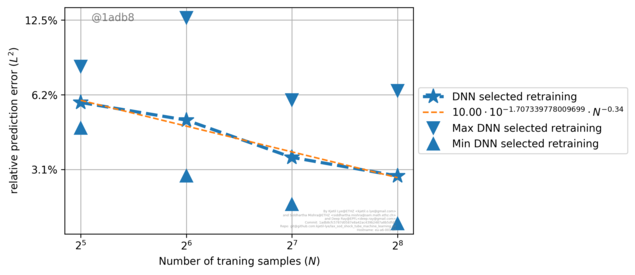
\includegraphics[width=0.48\textwidth]{img/laxsodtraining_size_prediction_l2_relative_q1_ordinary_onlyadamwithl2andlowregularizationorl1withregularizationbestperforming_sel_min_max_notitle.png}} 
\subfigure[Q2]{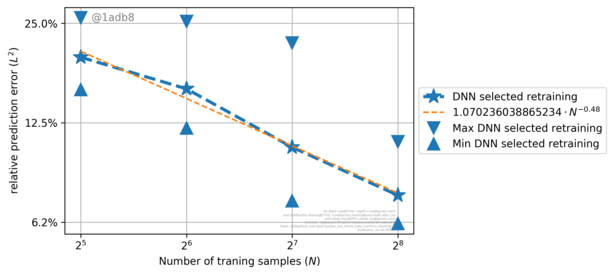
\includegraphics[width=0.48\textwidth]{img/laxsodtraining_size_prediction_l2_relative_q2_ordinary_onlyadamwithl2andlowregularizationorl1withregularizationbestperforming_sel_min_max_notitle.png}} 
\subfigure[Q3]{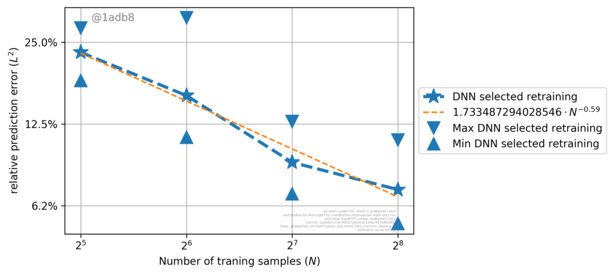
\includegraphics[width=0.48\textwidth]{img/laxsodtraining_size_prediction_l2_relative_q3_ordinary_onlyadamwithl2andlowregularizationorl1withregularizationbestperforming_sel_min_max_notitle.png}} 
\caption{LAX SOD Relative percentage mean square prediction error \eqref{eq:perr} (Y-axis) for the neural networks approximating the flow past airfoils problem, with respect to number of training samples (X-axis). For each number of training samples, we plot the mean, minimum and maximum (over hyperparameter configurations) of the prediction error. Only the selected (optimal) retraining is shown. }

\end{figure}




\begin{figure}
	\subfigure[Q1]{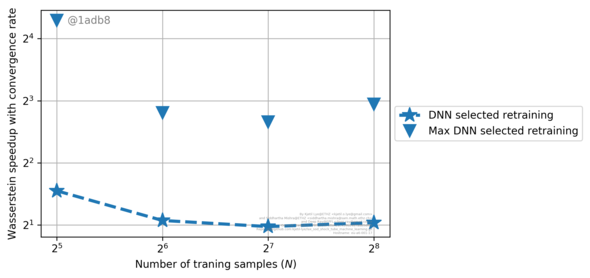
\includegraphics[width=0.5\textwidth]{img/laxsodtraining_size_wasserstein_speedup_real_q1_ordinary_allconfigurationsbestperforming_sel_max_notitle.png}} 
	\subfigure[Q2]{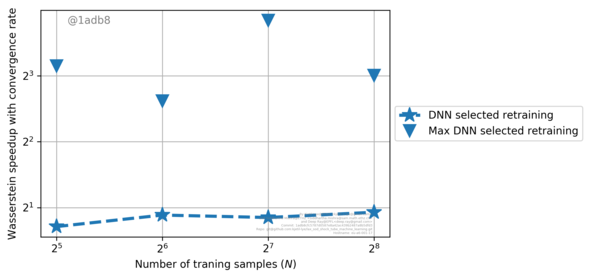
\includegraphics[width=0.5\textwidth]{img/laxsodtraining_size_wasserstein_speedup_real_q2_ordinary_allconfigurationsbestperforming_sel_max_notitle.png}} 
	\subfigure[Q3]{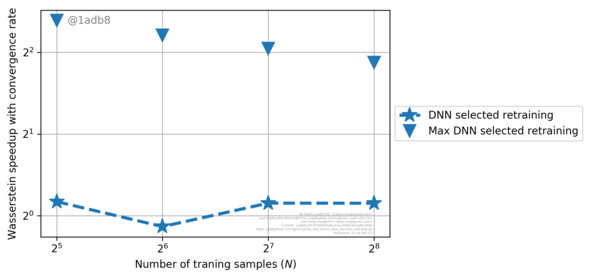
\includegraphics[width=0.5\textwidth]{img/laxsodtraining_size_wasserstein_speedup_real_q3_ordinary_allconfigurationsbestperforming_sel_max_notitle.png}} 
	\caption{LAX SOD Real speedups \eqref{eq:esp1} for the DLQMC algorithm over the baseline QMC algorithm (Y-axis) with respect to number of training samples (X-axis) for the flows past airfoils problem. The maximum and mean speed up (over all hyperparameter configurations)  are shown.}

\end{figure}
